\section{Konzept}
Das ist die Konzepteinleitung

\subsection{Anforderungen definieren}
Um die Anforderungen für das Spiel \textit{Stirnraten} zu erfassen, sollten zwei verschiedene Aspekte berücksichtigt werden: 

\begin{itemize}
	\item der \textbf{IST-Stand}, was muss mindestens erfüllt werden und 
	\item welche möglichen \textbf{Erweiterungen} entstehen durch eine API.
\end{itemize}

Um die Anforderungen greifbarer zu gestalten, wird auf das Prinzip von User Story Mapping zurückgegriffen. D.h. jede Anforderung ergibt sich aus einer sogenannte User Story. Diese ist so aufgebaut, dass beschrieben wird \textbf{wer} möchte \textbf{was} und \textbf{aus welchem Grund}.\cite{UserStoryMapping}\\

Im Folgenden gelten die zwei Definitionen: Ein Nutzer ist eine Person, welche die App spielt. Der Betreiber ist der Besitzer von Stirnraten. Ein User kann ein Nutzer oder Betreiber sein. \\

Ein Beispiel für eine User Story könnte lauten: Als Nutzer (\textit{wer}) möchte ich mein Spielprofil teilen (\textbf{was}), um mich besser mit meinen Freunden messen zu können ({\textbf{warum}).\\
	
Wie diese User Story nun umgesetzt wird, muss abgewogen werden. Zum einen sollten User Stories konkret genug formuliert werden, so dass klar ist, was der User möchte. Zum anderen bleibt bei der Entwicklung ein agiler Handlungsspielraum.\cite{UserStoryMapping} Eine Teile-Funkion beispielweise kann unterschiedlich aufwendig umgesetzt werden. Der Nutzer könnte ein Text teilen, ein extra aufbereitets Bild oder einen Link, welcher auf ein mögliches Online-Profile verweist. All diese Möglichkeiten bedeuten unterschiedliche Aufwände. Alternativ könnte man aus dieser einen User Story drei erstellen, welche entsprechend unterschiedlich priorisiert werden.\\

\textit{Exkurs - Spielprinzip Stirnraten: Die Spieleranzahl muss mindestens zwei betragen. Ein Spieler wählt aus verschiedenen Kategorien aus und hält sich das Telefon an die Stirn. Es erscheint Begriff, welchen der Gegenüber erklären muss. Errät der Spieler den Begriff, neigt er das Telefon nach vorne und ein neuer Begriff erscheint. Weiß er ihn nicht, kann er diesen überspringen, in dem er das Telefon nach hinten neigt. Ziel ist es, innerhalb einer frei wählbaren Zeit (z.B. 60 Sekunden), so viele Begriffe wie möglich zu erraten.}

\subsubsection{Erfassung Stirnratens IST-Stand}

In der folgenden Tabelle \ref{tab:bestehende_funktionen} wird gezeigt, welche Funktionen die App bereits auf dem Gerät bereitstellt, welche aber zukünftig serverseitig erledigt werden sollen. 

\begin{table}[H]
	\begin{center}
		\begin{tabular}{p{3cm}p{10cm}}
			Funktion & Beschreibung \\ \hline
			Profil/Statistik & Nach jedem Spiel werden verschiedene Daten erfasst, z.B. die Dauer des Spiels oder richtig geratene Wörter. Löscht man die App, ist dieses Profil unwiederbringlich. \\
			Bereitstellung Begriffe & Die über 6000 verschiedenen Begriffe liegen nur offline zur Verfügung. Editieren, Hinzufügen und Löschen geht nur über das Updaten der App.\\
			Zweisprachigkeit & Die App wird für den deutschen sowie den englischen Sprachraum angeboten. Es ist gewährleistet, dass je nach Nutzer, auf die sprachlich richtige Datenbank zugegriffen wird.\\
		\end{tabular}
	\end{center}
	\caption[bestehende Funktionen in Stirnraten]{bestehende Funktionen in Stirnraten}
	\label{tab:bestehende_funktionen} 
\end{table}

Aus dem IST-Zustand ergeben sich bereits folgende User Stories: 

\begin{itemize}
	\item Als Betreiber möchte ich neue Begriffe über eine Schnittstelle hinzufügen, editieren und löschen können, um die Datenbank schneller und leichter zu pflegen
	\item Als Betreiber möchte ich eine Datenbank, um nicht für zwei Apps (iOS und Android) den Datenbestand zu pflegen
	\item Als Betreiber möchte ich entscheiden können, in welcher Sprache (englisch oder deutsch) ich Begriffe manipuliere, um sinnvolle Daten zu gewährleisten
	\item Als Nutzer möchte ich das Spiel immer offline spielen können, da ich auf Reisen häufiger kein stabiles Internet habe
	\item Als Nutzer möchte ich mein Spielerprofil online speichern, um es auf anderen Geräten oder nach einer Neuinstallation abrufen zu können
	\item Als Nutzer möchte ich automatisch die Sprache angezeigt kriegen, welche für mich relevant ist, weil es mir sonst zu kompliziert ist
\end{itemize}

\subsubsection{Erweiterungen mittels User Story Mapping}

Durch das Einführen einer API bieten sich folgende Erweiterungsmöglichkeiten an:

\begin{itemize}
	\item Als Betreiber möchte ich neue Kategorien hinzufügen, editieren und löschen können, um das Nutzerangebot zu vergrößern
	\item Als Betreiber möchte ich Bilder pro Kategorie hinzufügen, editieren und löschen können, um ein sprechendes Bild für die Nutzer zu hinterlegen
	\item Als Betreiber möchte ich eine Kategorie als Premium kennzeichnen können, um Angebotsaktionen zu schalten
	\item Als Betreiber möchte ich eine Kategorie (de)aktivieren können, um sie immer zu einem sinnvollen Zeitpunkt anbieten zu können
	\item Als Betreiber möchte ich eine Registrierfunktion anbieten, um die Nutzer stärker an mich zu binden.
	\item Als Betreiber möchte ich die Nutzer abrufen, welche sich bei mir registriert haben, um einen Nutzerstamm aufzubauen
	\item Als Betreiber möchte ich Nutzer aus Datenschutzgründen löschen können
	\item Als Nutzer möchte ich mich in einer Rangliste mit anderen Nutzern vergleichen können, um zu sehen, wer in dem Spiel besser ist.
	\item Als Nutzer möchte ich die Spielerprofile von anderen Nutzern detailliert ansehen, um zu sehen, was ihnen gefällt 
	\item Als Betreiber möchte ich die Ranglisten-Namen der Nutzer manipulieren können, um unflätige Namen/Missbrauch zu verhindern.
	\item Als Betreiber möchte ich kummulitierte Daten aus den Nutzerstatistiken sehen, um Marktentscheidungen besser treffen zu können
	\item Als Betreiber möchte ich die Kategorien sortieren können, um die Anordnung für die Nutzer bestmöglich zu gestalten
	\item Als Betreiber möchte ich sehen, wenn ein Begriff bereits in der Kategorie ist, um die Datenqualität zu gewährleisten
	\item Als Nutzer möchte ich eigene Begriffe einreichen können, weil mir manche Begriffe oder Kategorien im Spiel fehlen
	\item Als Nutzer möchte ich sehen, wenn ein eingereichter Begriff bereits in einer Kategorie existiert, um Bescheid zu wissen
	\item Als Betreiber möchte ich eingereichte Begriffe zulassen oder ablehnen können, um den Datenbestand zu vergrößeren bzw. die Qualität zu gewährleisten 
	\item Als Betreiber möchte ich sehen, wann meine Nutzer zuletzt online waren, um ggf. Marketingmaßnahmen zu unternehmen
	\item Als Betreiber möchte ich, dass Nutzer-Zugangsdaten entsprechend gut verschlüsselt sind, um die Datensicherheit zu gewährleisten
\end{itemize}

Die folgende Auflistung sind User Stories, welche auch als Anforderungen entstanden sind, aber im Rahmen der Projektarbeit aufgrund von Aufwänden nicht umgesetzt werden können.

\begin{itemize}
	\item Als Betreiber möchte ich eine Newsletter-Funktion anbieten, um die Nutzer über Neuigkeiten zu informieren
	\item Als Nutzer möchte ich ein Profilbild hochladen, um mein Profil zu indiviualisieren
	\item Als Nutzer möchte ich mein Passwort zurücksetzen können, wenn ich es vergessen habe. 
	\item Als Betreiber möchte ich individuelle Animationen vom Server an den Nutzer weiterreichen können, um die Verspieltheit der App zu unterstreichen.
	\item Als Betreiber möchte ich Themes und Farbcodes online bereitstellen, um den Nutzern Individualsierungsmöglichkeiten schneller und leichter bereitzustellen 
	\item Als Betreiber möchte ich automatisiert, individuelle (Push)Nachrichten senden, um den Nutzer stärker zu binden
\end{itemize}

Aus den User Stories ergeben sich konkrete Abhängigkeiten zwischen den Microservices sowie klare Vorlagen für die Datenhaltung, z.B. benötigt der Nutzer mindestens einen eindeutigen Namen sowie ein Passwort. Die konkrete Umsetzung ist in FIGURE-VERLINKEN-AUF-KAPITEL-5.

\subsection{Macroarchitektonische Festlegungen von Technologien}
Wie bereits in 3.4.2 erwähnt, können durch makroarchitektonische Entscheidungen gewisse Vorteile erzielt werden, wie z.B. dass die Technologien zur Infrastruktur des Unternehmens und zu den Kompetenzen der Mitarbeiter passen. Ebenfalls können strategische Entscheidungen (z.B. ausschließlich Nutzen von Cloudtechnologien) die Makroarchitektur beeinflussen. Im Folgenden werden einige Technologien für `Stirnraten` makroarchitektonisch festgelegt. 

\subsubsection{Wahl der Datenbank}
Bei der Entscheidung, ob eine relationale oder schemalose (NoSQL) Datenbank verwendet wird, wurde sich für eine relationale entschieden. NoSQL Datenbanken sind häufig für spezielle Anwendungsfälle sinnvoll, z.B. wenn das Datenbankmodell sich häufig ändert oder ein hohes Maß an Skalierung notwendig ist. Diese Fälle sind für Stirnraten nicht absehbar, weshalb auf den etablierten Standard einer relationalen Datenbank gesetzt wird.\cite{kloeckner2015nosql_vs_relationale_datenbank}\\

Im Bereich der relationalen Datenbanken können verschiedene Technologien zur Umsetzung genutzt werden. Es wurde sich auf die derzeit (Stand Mai 2019) vier Populärsten Technologien konzentriert: Oracle (Rang 1), MSSQL (2), MySQL (Rang 3) und Postgres (Rang 4).\cite{dbengines2019ranking}  Oracle und MSSQL wurden für das Projekt ausgeschlossen, da diese kommerziell betrieben werden. Für Postgres und MqSQL wurde ein sogenanntes Proof of Concept erstellt, d.h. es wurde in einem einfachen Szenario eine Machbarkeit überprüft. Die Grundanforderungen war, dass MySQL und Postgres in verschiedenen Docker-Containern auf einer Maschine laufen können. Bei dem Proof of Concept hat sich gezeigt, dass es deutlich komplizierter ist, multiple Postgres Instanzen auf einer Maschine zu starten, da zusätzlich individuelle Scripts ausgeführt werden müssen.\cite{postgres2016}\\

Beim Erstellen von multiplen MySQL-Instanzen kam es zu keinerlei Problemen. Aufgrund des Rankings und der einfacheren technischen Implementierung durch das Proof of Concept wurde, sollen makroarchitektonisch die Microservices MySQL verwenden.

\subsubsection{Programmiersprachen, Darstellungsart, REST und Docker}
\textbf{Programmiersprachen}: Anfangs wurde erwähnt, dass aufgrund unternehmensstrategischer Gründe Entscheidungen darüber getroffen werden, welcher Technologiestack verwendet wird. In Hinblick auf die Programmiersprachen wird deshalb festgelegt, dass die Microservices im .net Framework in c\# entwickelt werden. Diese Sprache wird am besten von dem Entwickler beherrscht, so dass Wartbarkeit, Nachhaltigkeit und Pflege des Codes langfristig garantiert sind. Als zusätzliche Alternative ist kotlin ebenfalls erlaubt.\\

%Fußnote einfügen und auf mobile Kommunikation verweisen.
\textbf{Darstellungsart}: Das verwendete Datenformat beim Austausch von Daten ist JSON (JavaScript Object Notation). Alternativ wäre auch die Extensible Markup Language (XML) möglich, allerdings ist XML deutlich aufgeblähter und damit weniger leichtgewichtig. Zusätzlich lässt JSON sich leichter von den Programmiersprachen weiterverarbeiten.\cite{jsonxml2006heise}\\

\textbf{REST}: Die Kommunikation zwischen den Microservices wird so festgelegt, dass sie dem Representational State Transfer-Paradigma (REST) unterliegen. Eine Alternative zu REST wäre SOAP (Simple Object Access Protocol) in Kombination mit WSDL (Web Services Description Language). Da WSDL allerdings auf der Basis von XML arbeitet und SOAP deutlich komplexer und schwerer skalierbar ist als REST, wird es nicht verwendet. \cite{ayadi2008rest_vs_soap}\\ 

Die Prinzipien von REST sind bereits aus dem \textit{Modul Mobile Application Development} bekannt und werden deshalb nicht weiter erwähnt. \\

\textbf{Docker}: Neben Docker als Containerisierung existieren einige Alternativen wie Podman, Rocket, LXD, Flockport, Windocks oder Boxfuse. Sie unterscheiden sich teils in Sicherheitsaspekten, Preis, Kompatibilität zum Betriebssystem oder der Anbindung zu Kubernetes (Programm zum Bereitstellen, Skalieren und Verwalten von Container-Anwendungen).\cite{heise2019Podman}\cite{t3n2017Container} Es wurde sich für Docker entschieden. Zum einen da dies - wie bereits bei den Programmiersprachen - eine beherrschte Technologie ist. Zum anderen - gemessen am Google Trend - ist Docker die bevorzugt gesuchte Technologie für Containerisierung:  

\begin{figure}[ht]
	\centering
	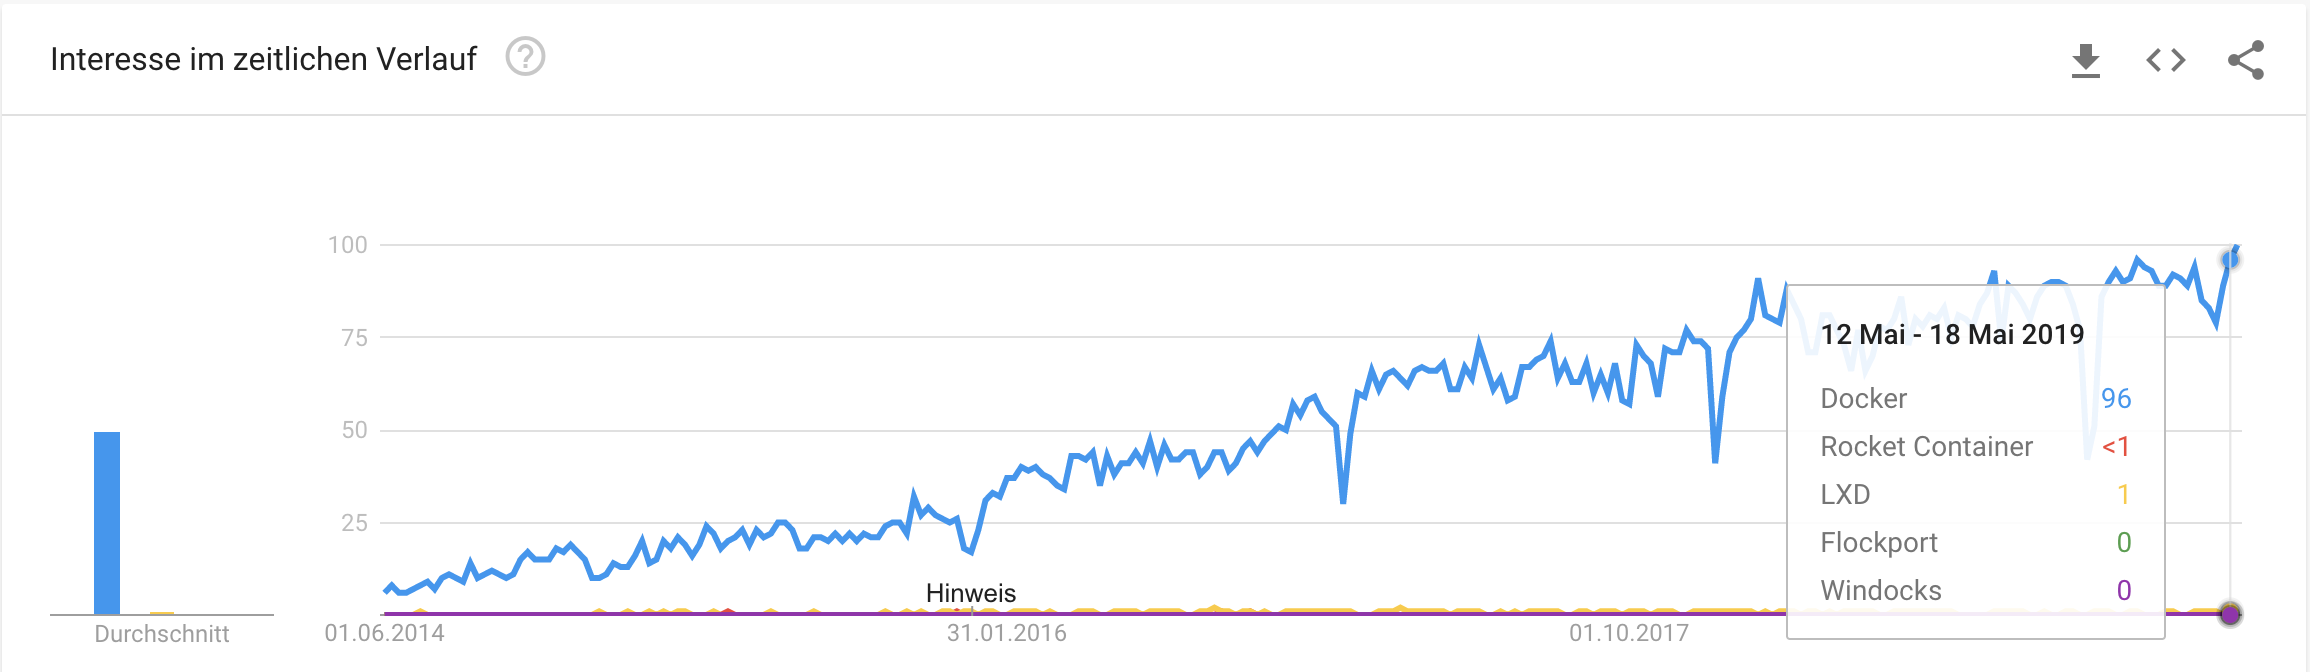
\includegraphics[width=0.5\textwidth]{docker_google_trend}
	\caption[Docker Google Trends] {Trends bei den Suchworten: Docker, Rocket Container, LXD, Flockport und Podman}
	\label{fig:docker_google_trends}
\end{figure}


\subsubsection{Bounded Contexts - Architektur des Projektes}

Aus den Abschnitt \ref{sec:domain_driven_design} lassen sich folgende Bounded Contexts erstellen: 

\begin{figure}[ht]
	\centering
	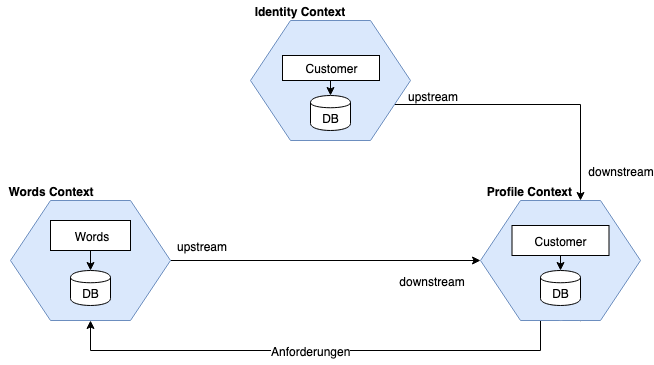
\includegraphics[width=0.6\textwidth]{ddd_context}
	\caption[Bounded Contexts für Stirnraten] {Bounded Contexts für die Stirnraten API.}
	\label{fig:ddd_context}
\end{figure}

Durch die verschiedenen Kontexte lassen sich entsprechende Microservices abbilden. Zusätzlich wird definiert, was unter welchen Fachtermini im entsprechenden Context zu verstehen ist. Zum Beispiel stellt der \textit{Identity Context} dem Nutzer ein Token aus mit dem er weitere Aktionen ausführen darf. Dafür speichert der \textit{Identity Context} sich in seinem Customer-Modell (Domänenmodell) einen Namen und ein Passwort. Der Customer im \textit{Profile Context} dagegen enthält noch weitere Informationen wie z.B. Anzahl der gespielten Spiele, geratene Begriffe, Lieblingskategorie und Spielminuten. Der Customer im \textit{Rank Context} benötigt dagegen nur den Customer-Namen und noch zu definierende Parameter aus denen Customer-Punkte generiert werden können, um eine Bestenliste darzustellen.\\

Es wurde bereits erwähnt, dass der \textit{upstream} dem \textit{downstream} Informationen bereitstellt. Zusätzlich können Anforderungen gestellt werden, damit mit den Daten, die der \textit{downstream} erhält, entsprechend gerarbeitet werden kann. In der Abbildung \ref{fig:ddd_context} fordert der \textit{Profile Context} Informationen vom \textit{Words Context} sowie der \textit{Rank Context} vom \textit{Profile Context}  \\

Um die aus den User Stories entstanden Anforderungen zu erfüllen, werden im Folgenden die Domainmodels konzeptioniert. Diese können während der Implementierungsphase noch abweichen. \\

\underline{Words-Context: Words Domainmodel}\\
\textit{id}: Dient als unique identifier\\
\textit{category\_name}: Name der Kategorie\\
\textit{subtitle}: Optionale Beschreibung der Kategorie\\
\textit{image\_name}: Name des Bildes, welches für eine Kategorie hinterlegt werden soll\\
\textit{premium\_key}: Notwendig für die Kaufabwicklung zum Identifizieren, um welchen In-App-Kauf es sich handelt\\
\textit{is\_premium}: Markiert, ob eine Kategorie kostenpflichtig ist oder nicht\\
\textit{selected}: Definiert, ob die Kategorie in der App vorausgewählt ist oder nicht\\
\textit{words}: Die Begriffe pro Kategorie, welche erraten werden können\\
\textit{sort}: Definiert, an welcher Stelle in der Sortierung die Kategorie ist\\
\textit{is\_activ}: Definiert, ob die Kategorie in der App angezeigt wird oder nicht\\
\textit{updated\_at}: Zeitpunkt, wann die Kategorie das letzte mal verändert worden ist \\

\underline{Identiy-Context: Customer-Domainmodel}:\\
\textit{id}: Dient als unique identifier \\
\textit{name}: Name des Benutzers\\
\textit{password}: Passwort des Benuzters\\

\underline{Profile-Context: Customer-Domainmodel}:\\
\textit{id}: Dient als unique identifier \\
\textit{name}: Name des Benutzers (kommt aus dem Identiy-Context)\\
\textit{mail}: E-Mail-Adresse des Benutzers (optional)\\
\textit{played\_games}: Zeigt die Anzahl absolvierter Spiele\\
\textit{most\_right\_words}: Zeigt die Anzahl der Wörter, die während einer Runde geraten worden sind\\
\textit{most\_skipped\_words}: Zeigt die Anzahl der Wörter, die während einer Runde übersprungen worden sind\\
\textit{right\_words}: Zeigt Anzahl aller Wörter, die richtig geraten worden sind\\
\textit{skipped\_words}: Zeigt Anzahl aller Wörter, die übersprungen worden sind\\
\textit{time}: Zeigt, wie lange der Benutzer gespielt hat \\
\textit{top\_categories}: Speichert, welche Kategorien der Benutzer favorisiert\\

\underline{Rank-Context: Customer-Domainmodel}:\\
\textit{id}: Dient als unique identifier \\
\textit{name}: Name des Benutzers (kommt aus dem Identiy-Context)\\
\textit{played\_games}: Zeigt die Anzahl absolvierter Spiele (kommt aus Profile-Context)\\
\textit{right\_words}: Zeigt Anzahl aller Wörter, die richtig geraten worden sind (kommt aus Profile-Context)\\
\textit{skipped\_words}: Zeigt Anzahl aller Wörter, die übersprungen worden sind (kommt aus Profile-Context)\\
\textit{time}: Zeigt, wie lange der Benutzer gespielt hat (kommt aus Profile-Context)\\
\textit{points}: Punkte, die sich aus played\_games, right\_words, skipped\_words und time berechnen \\

Es lässt sich feststellen, dass es Überschneidungen zwischen dem Customer-Domainmodel gibt, je nach dem in welchem Kontext man sich befindet. Natürlich verändert dieses Konzept sich noch im Laufe der Produktentwicklung und muss iterativ an den Stand der Entwicklung angepasst werden. Ebenfalls gilt zu erwähnen, dass es an dieser Stelle im Domain Driven Design nicht zwangsweise ein richtig oder falsch gibt. Dies ist ein Konzeptentwurf, aber natürlich nicht die einzige mögliche Lösung.

\subsection{Wahl des API-Gateway}
- Ocelot % (leichtgewichtig und open source (https://devblogs.microsoft.com/cesardelatorre/designing-and-implementing-api-gateways-with-ocelot-in-a-microservices-and-container-based-architecture/), empfohlen von Microsoft für .net)
- Eigenbau  (%https://medium.com/streamwriter/api-gateway-aspnet-core-a46ef259dc54 Aufwand, vermutlich qualitativ nicht so gut, Umfang nicht gegebn, Vorteile: Man weiß, was passiert)
- welches gibt es noch?  %- Ggf. Cloud ApiGateway (von entsprechenden Größen AWS usw.)

% Artikel lesen und Grundlagen rausarbeiten: https://docs.microsoft.com/de-de/dotnet/standard/microservices-architecture/secure-net-microservices-web-applications/

% Guter Artikel bzgl. OAuth2: https://medium.com/google-cloud/understanding-oauth2-and-building-a-basic-authorization-server-of-your-own-a-beginners-guide-cf7451a16f66

\subsection{Wahl der Kommunikation}
- Erwähnen, dass asynchrone Kommunikation verwendet wird, aufgrund der Vorteile aus den Grundlagen 
- Technologie: Masstransit (RabbitMQ) vs. Kafka

\subsection{Wahl der Authenfizierung/Authorisierung}
- Auth0
- OAuth2: Authentication Framework (mit OpenId Connect?) -> Spricht die Zeit, Komplexität und so eine Komplexität gar nicht benötigt 
- JWT: Also Protocol
- Dritteranbieter Dienst -> Auth0 (zu teuer)
- ggf. ohne OAuth

